\subsection{Lidar Mount}
% Design reqs: needed to rigidly attach to Nao for data transformation purposes, needed to see forward,
% lightweight, Nao needed to be able to move his head while wearing it,
% needed to be able to use the sonars (just in case).
In order to attach the URG Lidar to the Nao a custom Lidar mount was built.
The mount needed to hold the Lidar such that obstacles in front of the robot
could be sensed. The mount needed to be lightweight, rigidly attached, and allow
the robot to move its head to track the red cube. It should also not inhibit
the use of the sonars, in the event that the sonars are used in the future.

% Mounting it to the head seemed like it was going to be tough, so a vest was designed.
% Straps and foam seemed like they'd hold well enough. In fact they hold so well I can lift Nao up by the mount.
% The mount was made from PLA, 3D printer, foam, velcro straps.
As the Nao is not equipped with any mounting points, the Lidar mount was 
designed as a tray mounted to the front of the robot at waist-height, attached
using straps. The rigid parts were manufactured out of PLA plastic using a 3D
printer. The rigid parts that would contact the robot were padded with foam to
create a surface that would conform to the Nao's body and hold securely.
Figure~\ref{fig:nao_lidar_mount_nao_dimetric1} shows a CAD model of the finished
assembly.
A picture of the assembly mounted to the robot can be seen in
Figure~\ref{fig:nao_lidar_mount_picture1}.

\begin{figure}
\centering
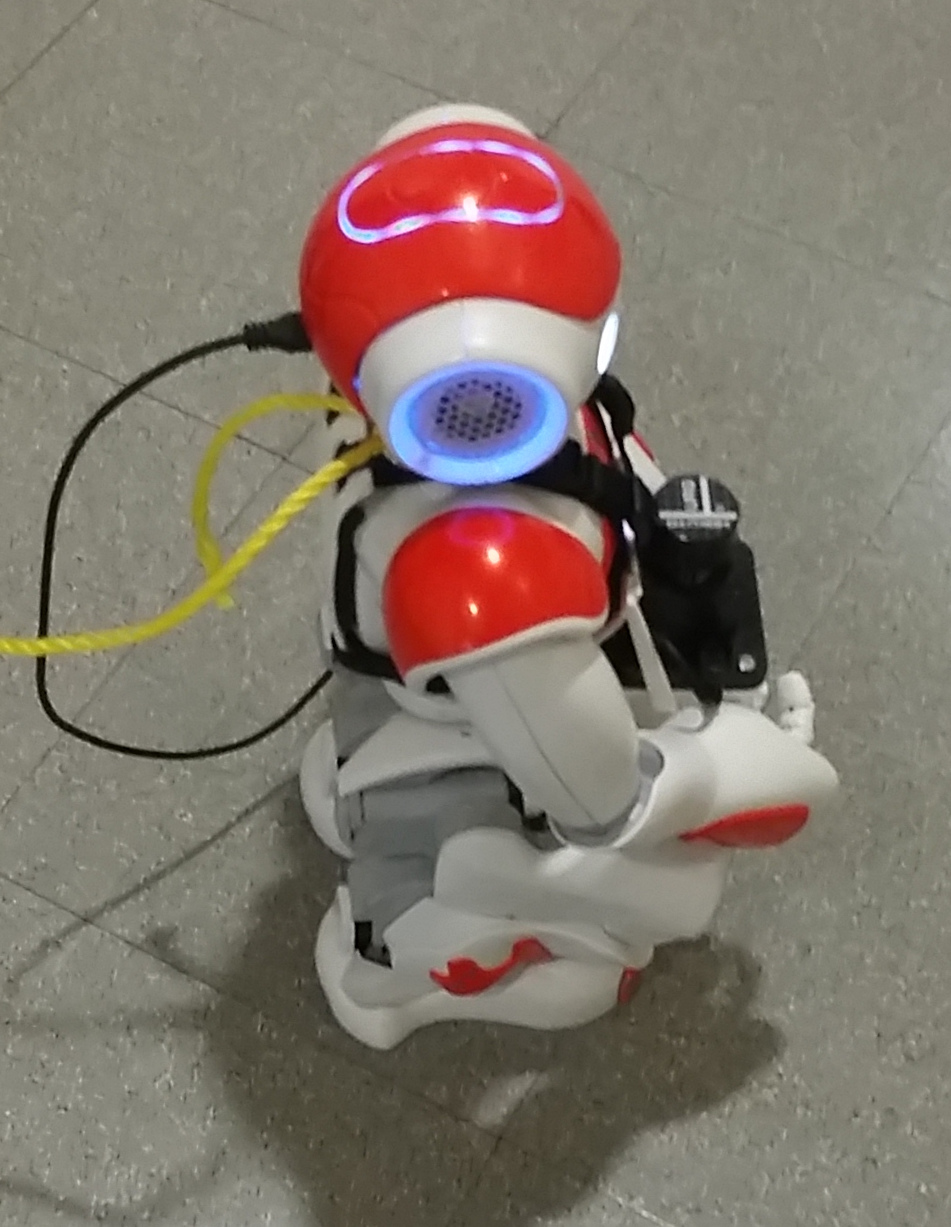
\includegraphics[height=0.4\textheight]{backpack/nao_with_mount2.jpg}
\caption{Figure showing a photograph of the URG mounted to the Nao using the
         custom Lidar mount.}
\label{fig:nao_lidar_mount_picture1}
\end{figure}

\begin{figure}
\centering
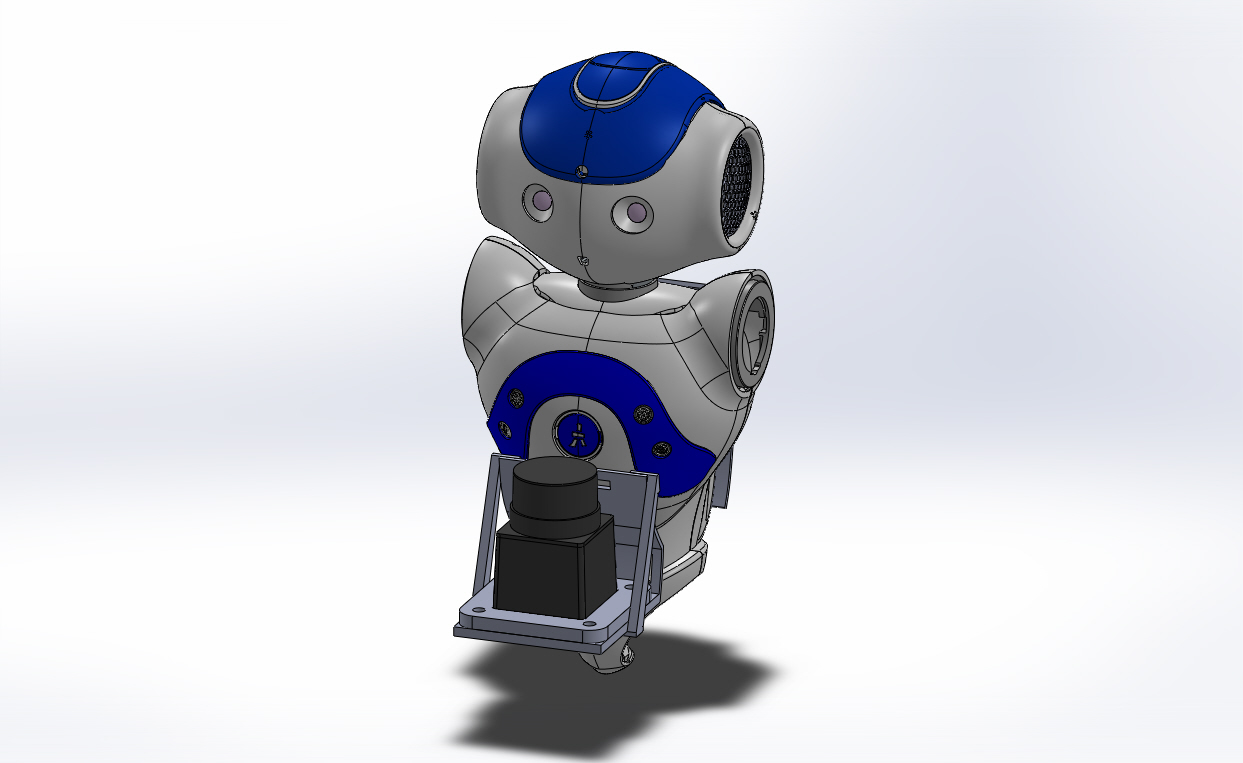
\includegraphics[height=0.4\textheight]{backpack/Assem_Nao_Dimetric1.jpg}
\caption{Figure showing CAD model of Nao with Hokuyo URG-04LX-UG01 mounted
         to the waist of the robot using a custom mount.}
\label{fig:nao_lidar_mount_nao_dimetric1}
\end{figure}

\begin{figure}
\centering
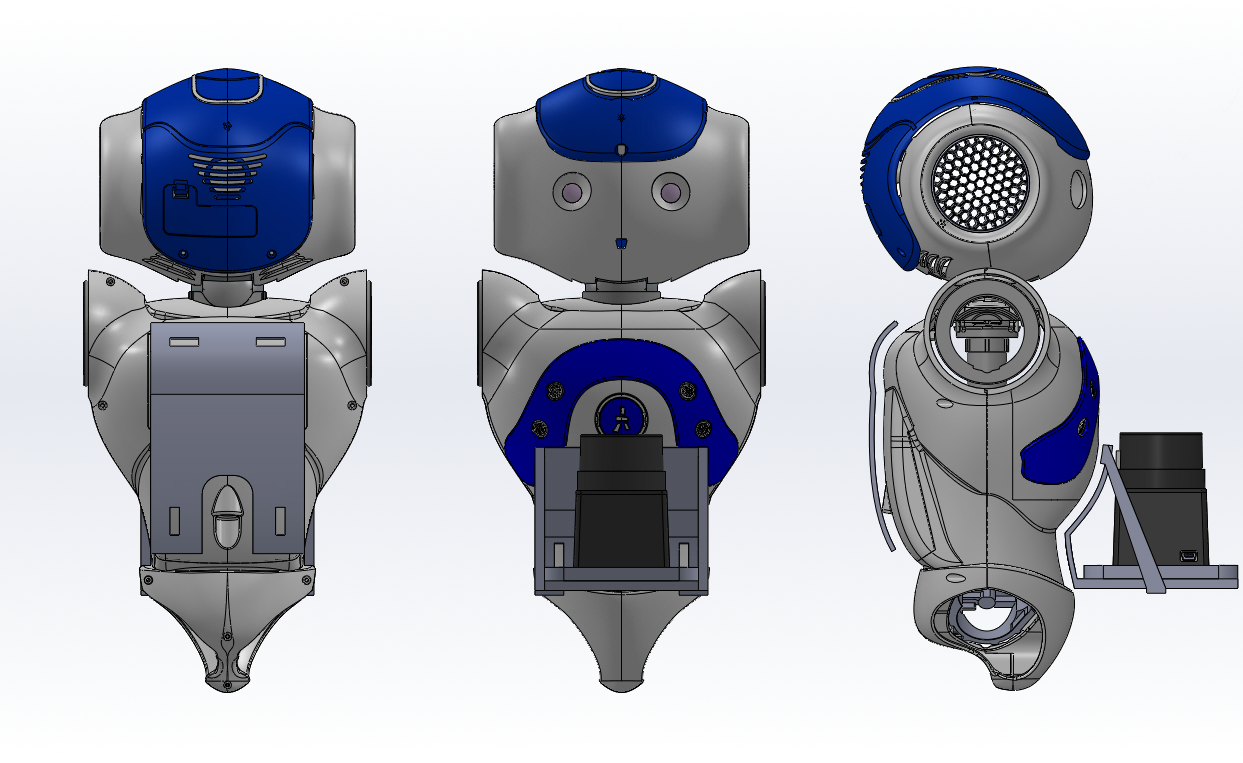
\includegraphics[height=0.4\textheight]{backpack/Assem_Nao_Three_View1.png}
\caption{Figure showing back, front, and side views of the URG CAD model 
         mounted to the Nao using the custom mount.}
\label{fig:nao_lidar_mount_nao_three_view1}
\end{figure}

The front subassembly of the Lidar mount consists of three parts: a front plate,
a base plate, and side supports. Figure~\ref{fig:nao_lidar_mount_dimetric1}
shows a CAD model of the assembled front subassembly with the URG installed.

\begin{figure}
\centering
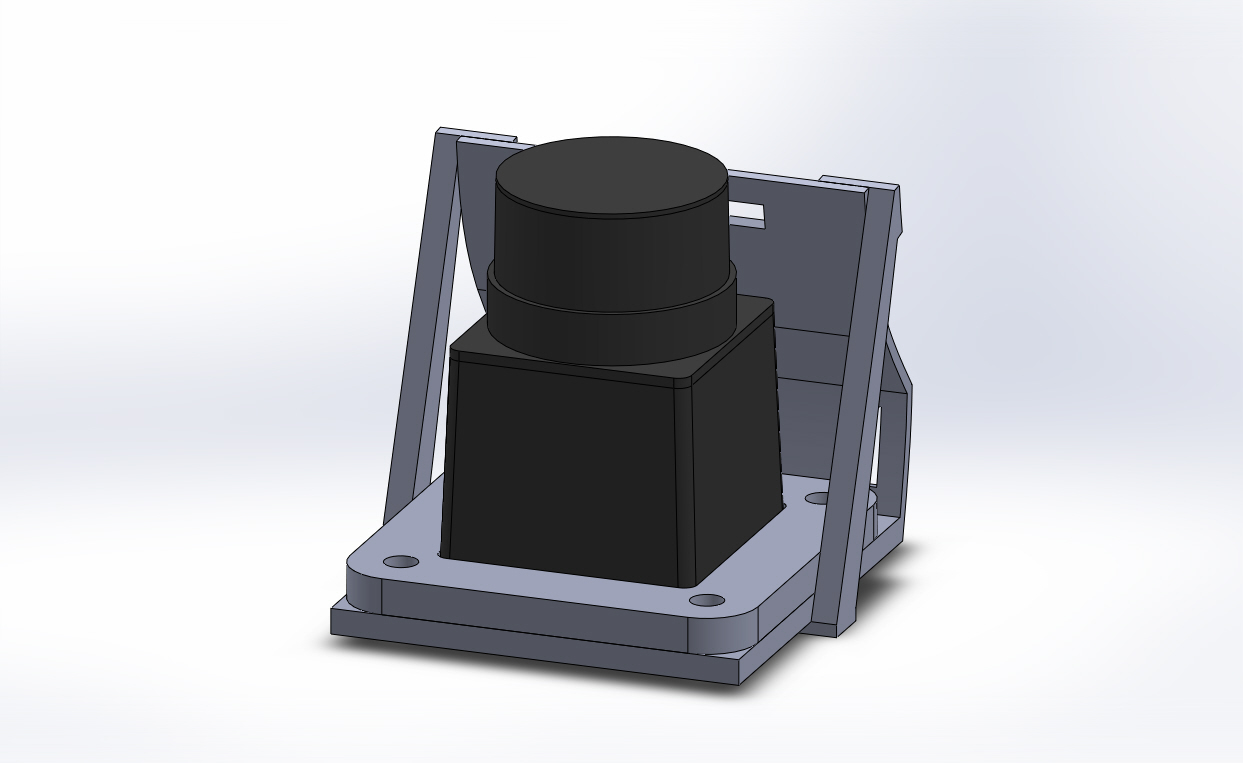
\includegraphics[height=0.4\textheight]{backpack/Assem_FrontOnly_Dimetric1.jpg}
\caption{Figure showing CAD model of the URG attached to the front subassembly
         of the custom Lidar mount.}
\label{fig:nao_lidar_mount_dimetric1}
\end{figure}

\begin{figure}
\centering
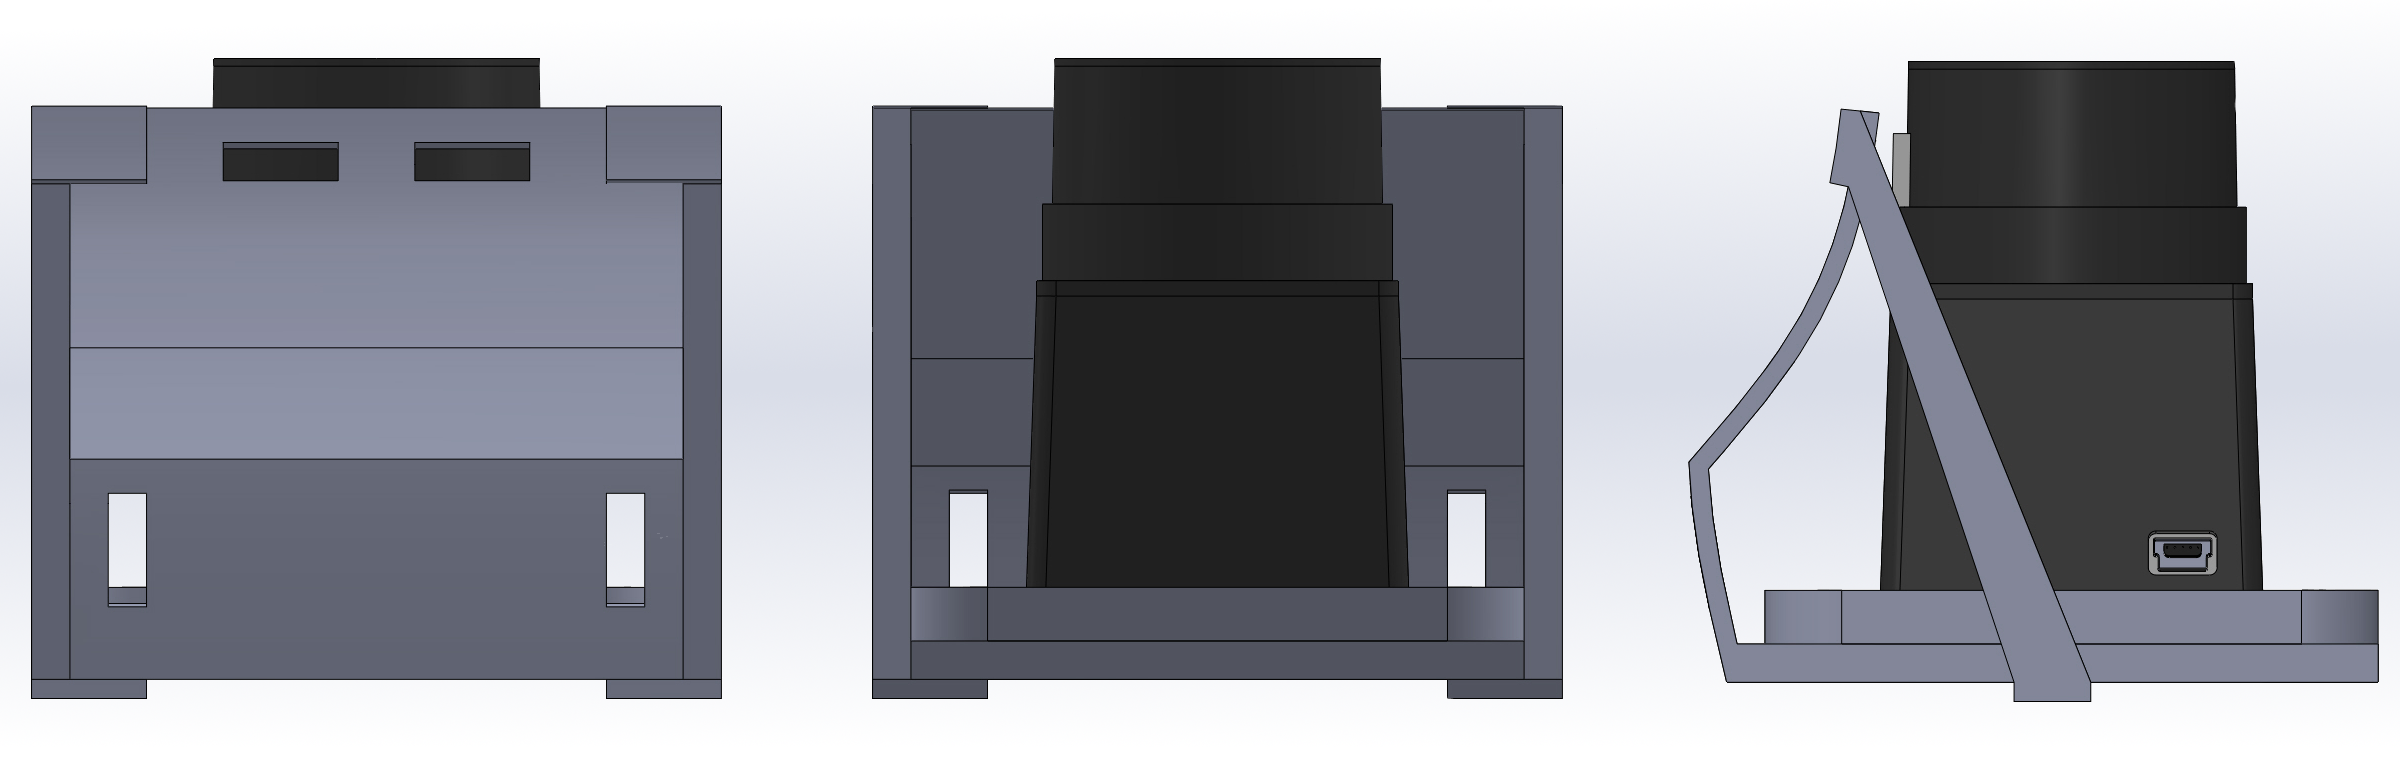
\includegraphics[width=\textwidth]{backpack/Assem_FrontOnly_Three_View1.png}
\caption{Figure showing back, front, and side views of the URG CAD model
         attached to the front subassembly of the custom mount.}
\label{fig:nao_lidar_mount_three_view1}
\end{figure}

The front plate has a shape that follows the form of the Nao.
It is padded with foam that is glued to the plate to conform to the robot more
closely and minimize the effects of vibration.
Figure~\ref{fig:nao_lidar_mount_frontplate_trimetric1} shows a CAD model of the
front plate. It has a tray that projects perpendicular from the robot to hold 
the base plate. Two mounting holes on the tray secure the base plate to the tray.
The front plate is secured to the robot via four rectangular holes which receive
velcro straps that go to the back plate. These straps are tightened to hold the
Lidar mount to the robot.

\begin{figure}
\centering
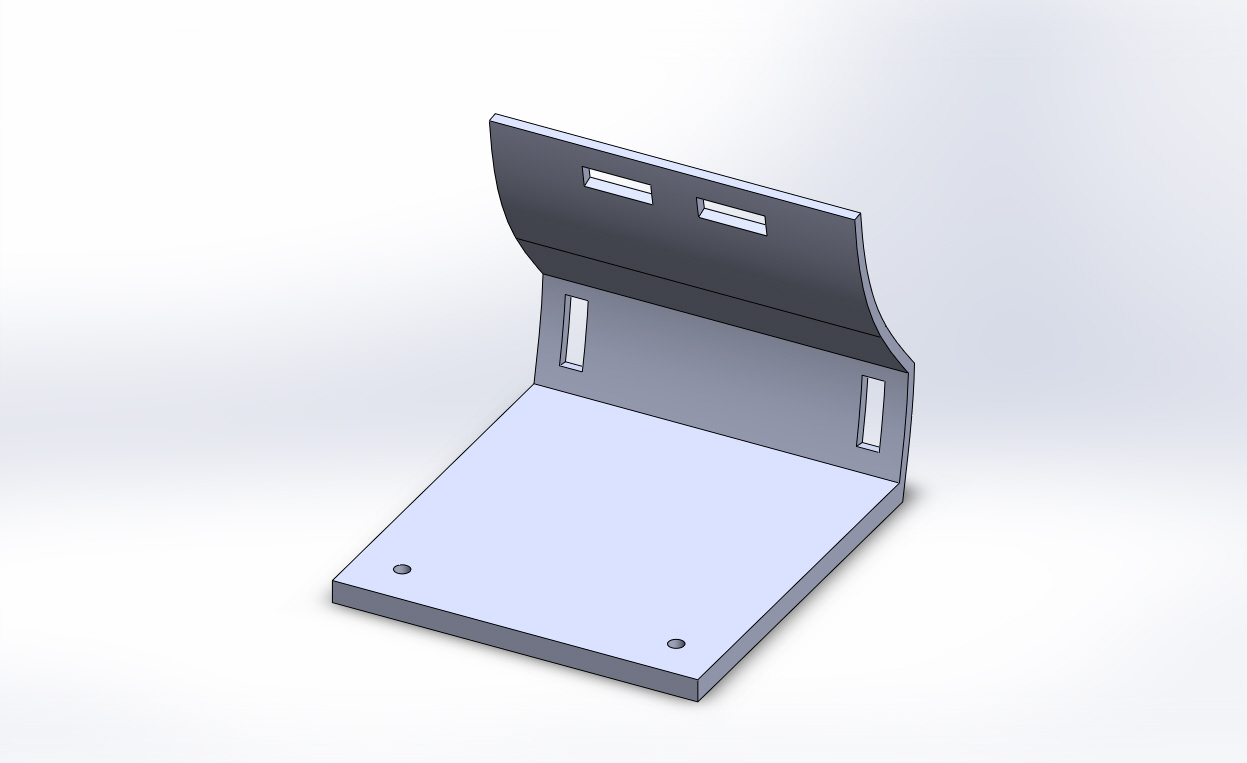
\includegraphics[height=0.4\textheight]{backpack/Front_Plate_Trimetric1.jpg}
\caption{Figure showing a CAD model of the front plate of the custom Lidar
         mount. The base plate attaches to this plate.}
\label{fig:nao_lidar_mount_frontplate_trimetric1}
\end{figure}

\begin{figure}
\centering
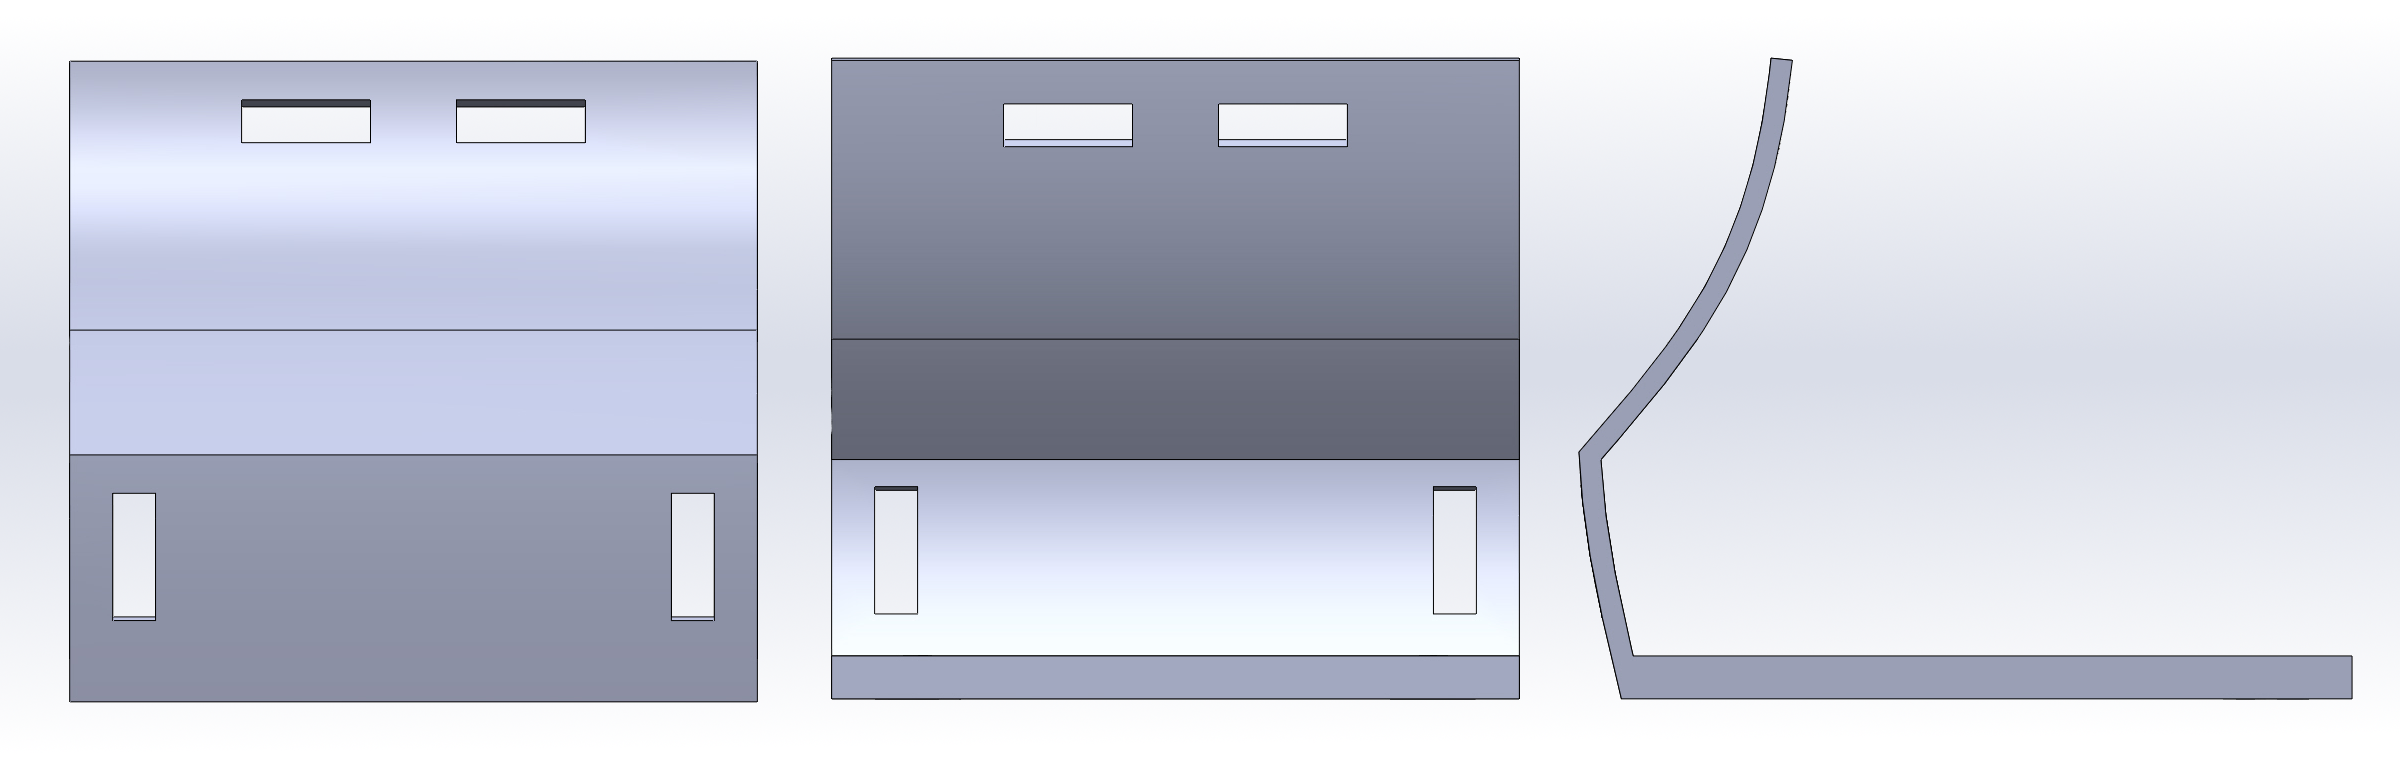
\includegraphics[width=\textwidth]{backpack/Front_Plate_Three_View1.png}
\caption{Figure showing back, front, and side views of the CAD model of the
         front plate.}
\label{fig:nao_lidar_mount_frontplate_three_view1}
\end{figure}

The URG is attached to the base plate, which in turn is attached to the 
tray of the front plate. The URG is attached to this intermediate part
rather than directly to the front plate to facilitate the mechanical
interoperability of different sensors to the front plate without needing
to produce different front plates for different sensors. Instead, different
base plates are made for different sensors. For example, the lower cost
RPLidar \cite{rp_lidar} or the VLP-16 Puck 3D Lidar
\cite{puck_lidar} are alternative Lidars that could
be mounted to the Nao for experimentation but have a different mounting 
configuration than the URG\@. In this way, new base plates can be manufactured
rather than front plates, allowing for a more modular design.

\begin{figure}
\centering
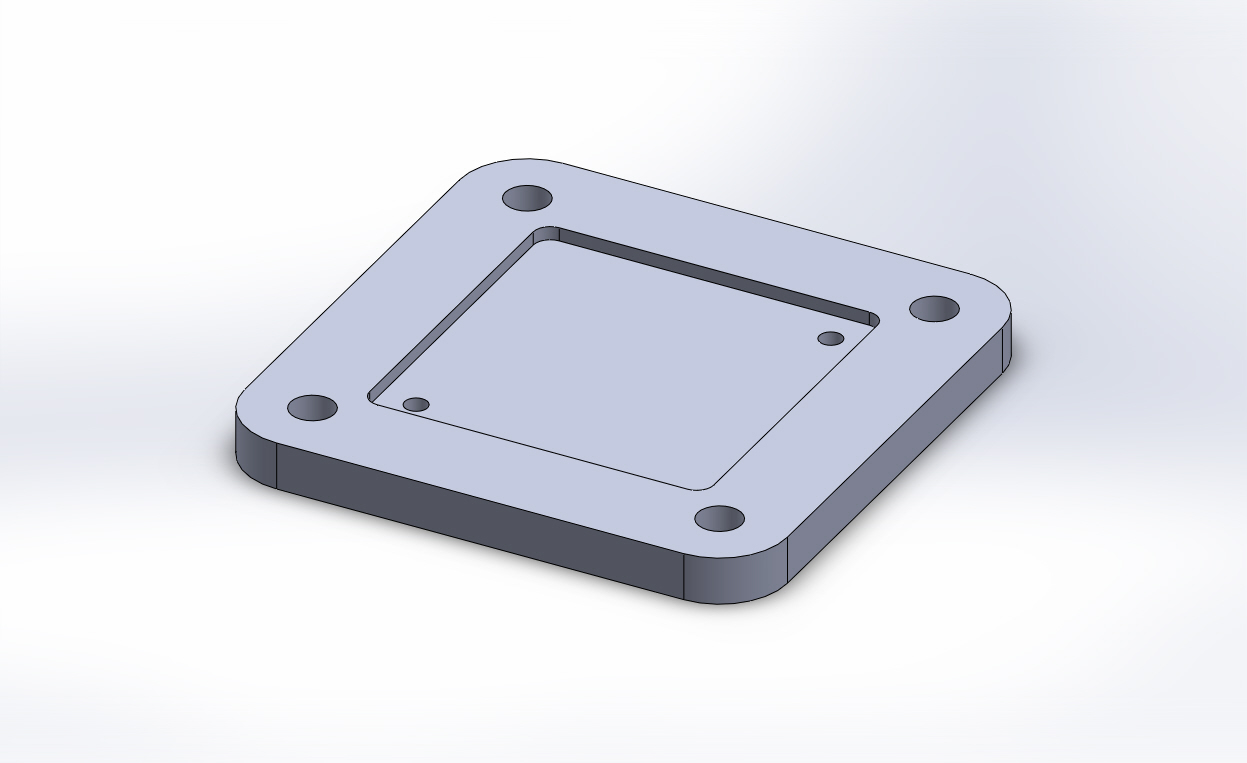
\includegraphics[height=0.4\textheight]{backpack/Base_Plate_Trimetric1.jpg}
\caption{Figure showing a CAD model of the base plate of the custom Lidar
         mount. The base plate is part of the front subassembly.
         The URG attaches to this plate.}
\label{fig:nao_lidar_mount_baseplate_trimetric1}
\end{figure}

\begin{figure}
\centering
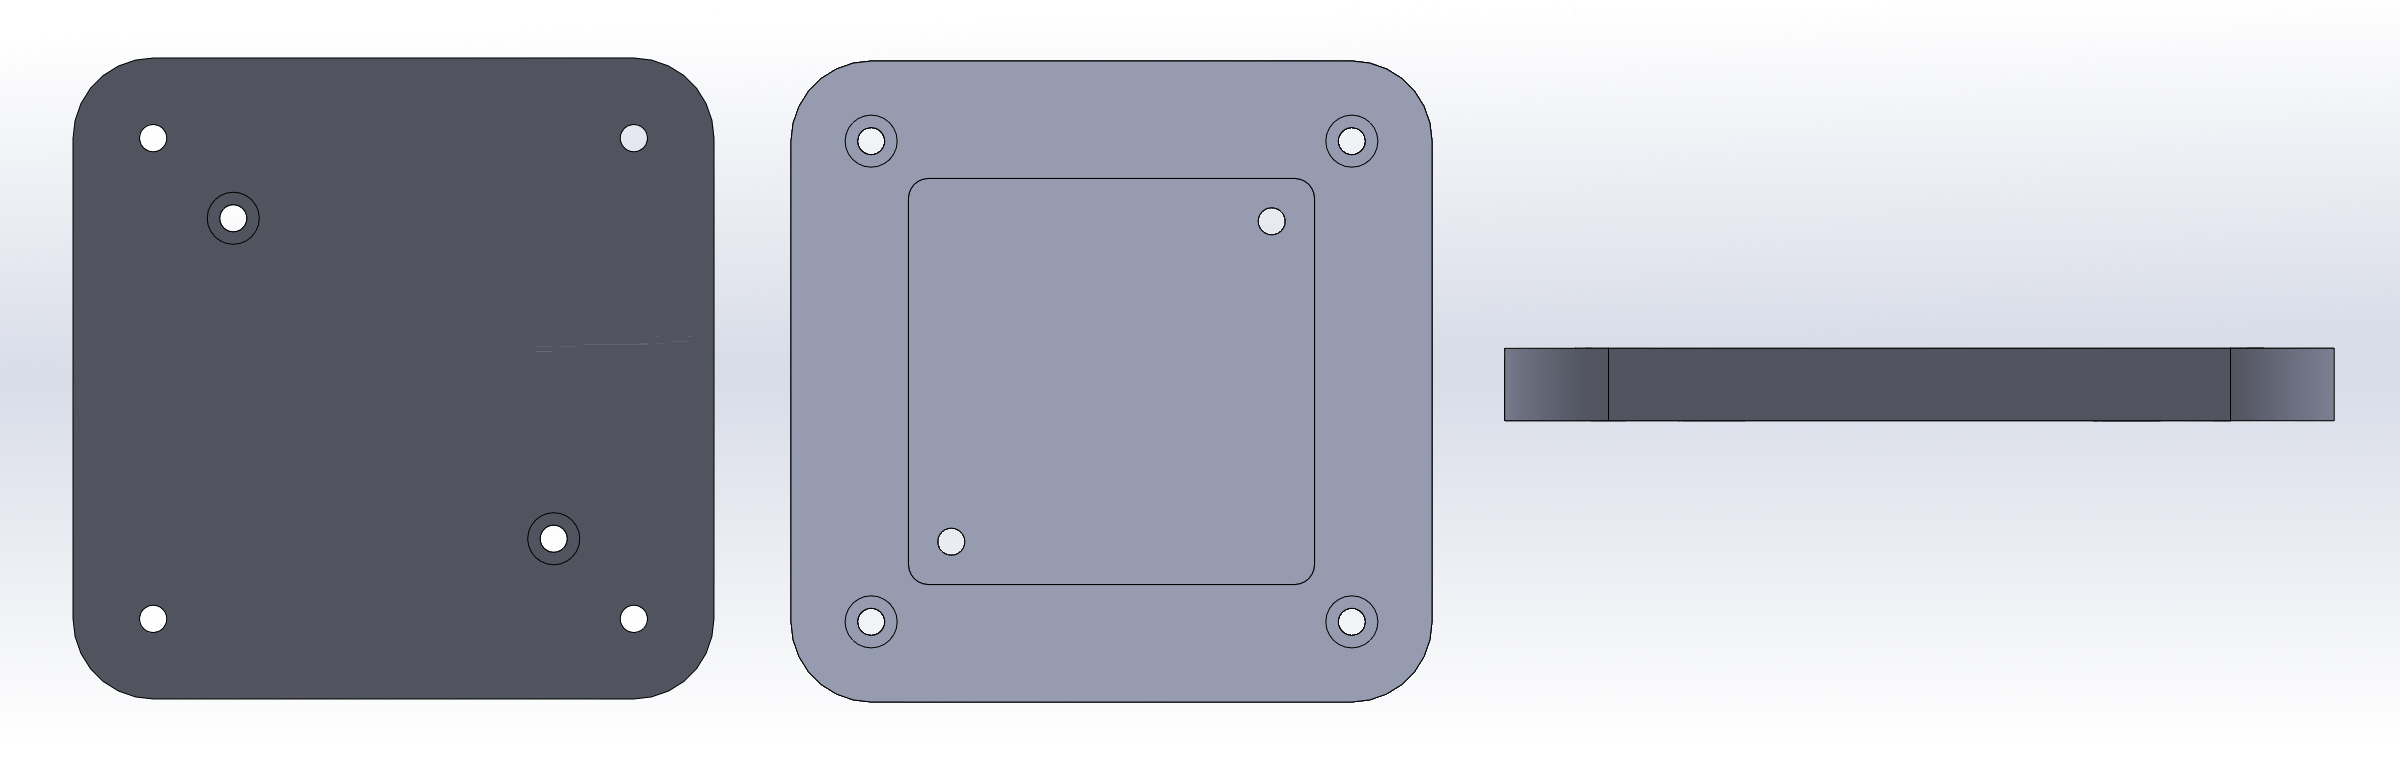
\includegraphics[width=\textwidth]{backpack/Base_Plate_Three_View1.png}
\caption{Figure showing back, front, and side views of the CAD model of the
         base plate.}
\label{fig:nao_lidar_mount_baseplate_three_view1}
\end{figure}

\begin{figure}
\centering
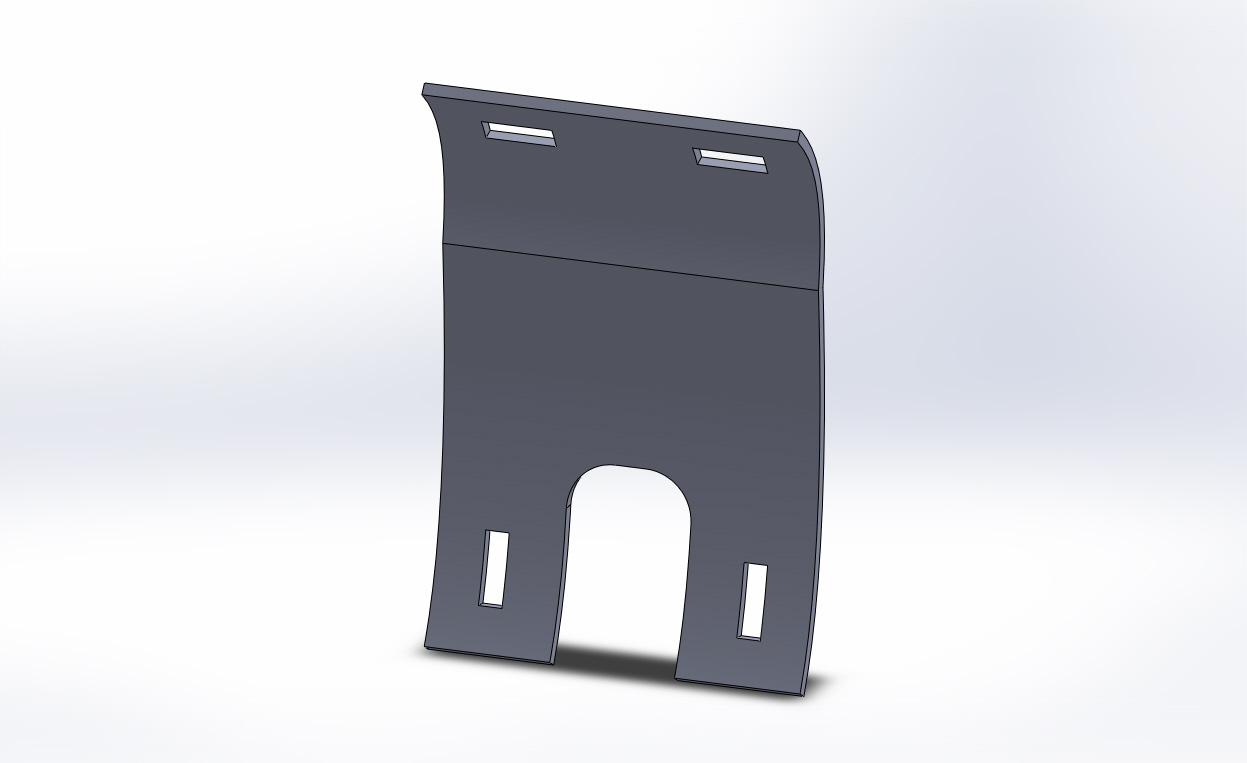
\includegraphics[height=0.4\textheight]{backpack/Back_Plate_Dimetric1.jpg}
\caption{Figure showing a CAD model of the back plate of the custom
         Lidar mount.}
\label{fig:nao_lidar_mount_backplate_dimetric1}
\end{figure}

\begin{figure}
\centering
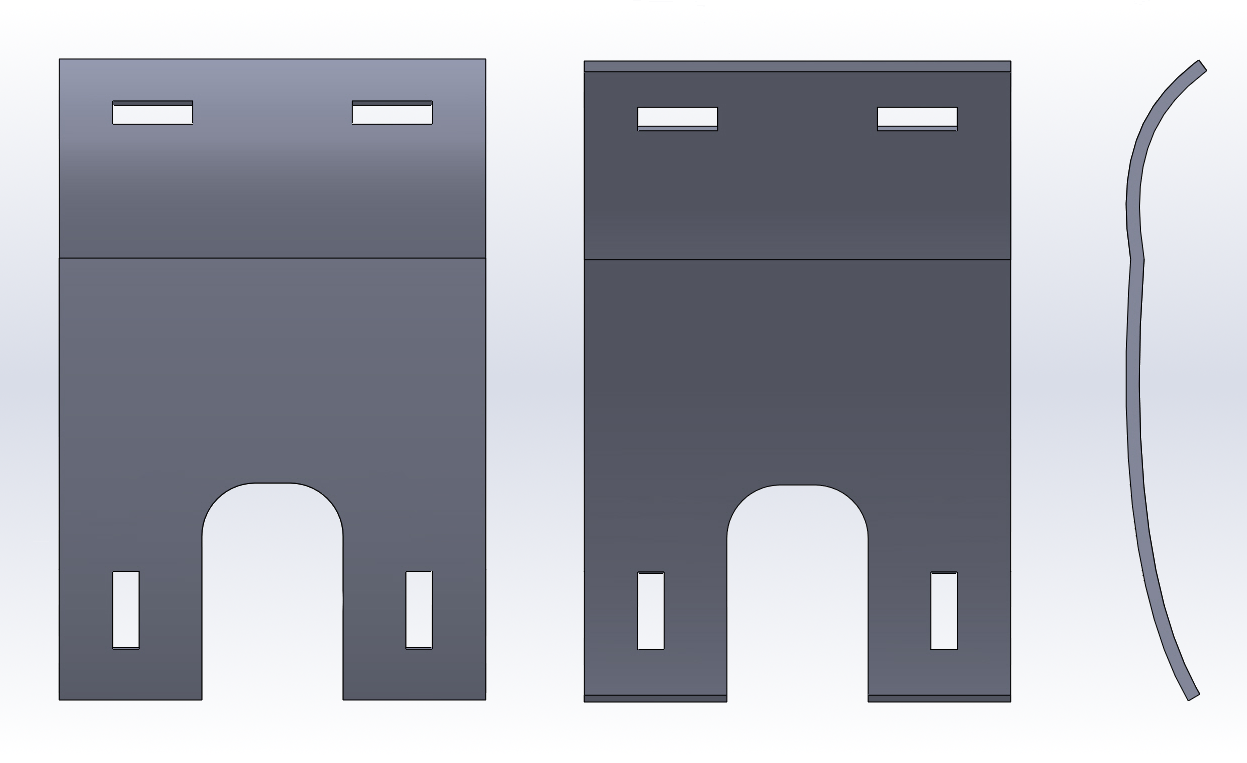
\includegraphics[width=\textwidth]{backpack/Back_Plate_Three_View1.png}
\caption{Figure showing back, front, and side views of the CAD model of the
         back plate of the custom Lidar mount.}
\label{fig:nao_lidar_mount_backplate_three_view1}
\end{figure}



\begin{figure}
\centering
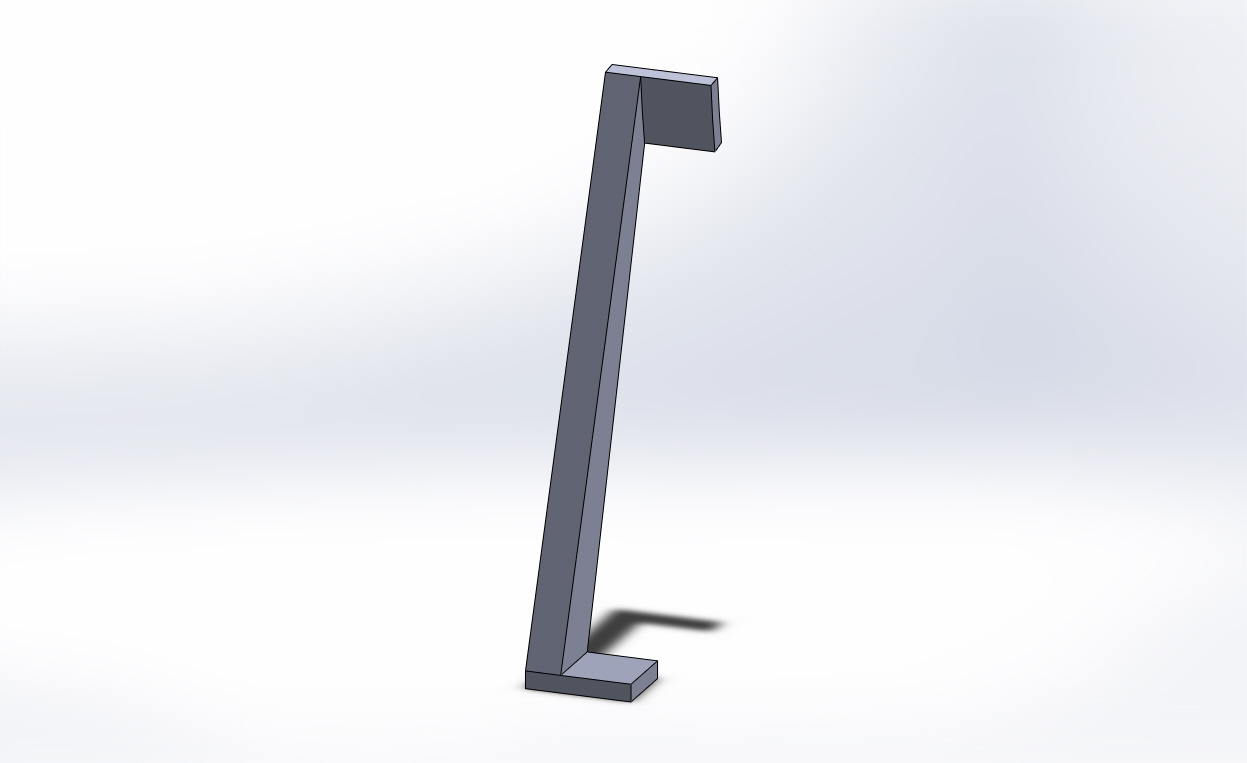
\includegraphics[height=0.4\textheight]{backpack/Support_Left_Trimetric1.jpg}
\caption{Figure showing a CAD model of the left side support of the custom
         Lidar mount. This support is bonded to the front plate to add rigidity
         to the front plate. The right side support is a mirror image of this
         part.}
\label{fig:nao_lidar_mount_supportleft_trimetric1}
\end{figure}

\begin{figure}
\centering

\includegraphics[height=0.4\textheight]{backpack/Support_Left_Three_View1.jpg}
\caption{Figure showing back, front and side views of the CAD model of the left
         side support.}
\label{fig:nao_lidar_mount_supportleft_three_view1}
\end{figure}
